\documentclass[12pt]{article}
\usepackage{amsmath,amsthm,amsfonts,amssymb, xcolor,enumerate,enumitem,xfrac,tikz,comment, pgfplots,soul, mathtools}
\usetikzlibrary{shapes.geometric,positioning,calc}
\usepackage{url}
\usepackage[colorlinks=true,
            linkcolor=blue,
            filecolor=magenta,
            urlcolor=black,
            citecolor=magenta,
            pdftitle={Reviewing report},
            pdfpagemode=FullScreen,
           ]{hyperref}

\newcommand{\R}{\mathbb{R}}
\newcommand{\Norm}[1]{\left|\left|  #1   \right|\right|}
\newcommand{\E}{\mathbb{E}}
\newcommand{\FoxH}[5]{H_{#2}^{#1}\left(#3\:\middle\vert\: \begin{subarray}{l}#4\\[0.4em] #5\end{subarray}\right)}
\newcommand{\ud}{\ensuremath{\mathrm{d}}}

\begin{document}

\title{Some symbolic tools for the {F}ox {$H$}-function}
\author{Le Chen                             \\
  Department of Maathematics and Statistics \\
  Auburn University                         \\
\url{le.chen@auburn.edu}, \url{chenle02@gmail.com}
}

\maketitle

In this note, we explain the code for checking the conditions of the Fox
$H$-function~\cite{fox:61:g}. Here we follow the notation from Kilbas and
Saigo~\cite{kilbas.saigo:04:h-transforms}.


Let $m,n,p,q$ be configure integers such that
\begin{align*}
  0 \le m \le q \quad \text{and} \quad
  0 \le n \le p.
\end{align*}
Let $a_i,b_j\in \mathbb{C}$ and $\alpha_i, \beta_j \in\R_+$ be the parameters given below:
\begin{center}
\renewcommand{\arraystretch}{1.2}
  \begin{tabular}{|c|cc|c|}
    \hline
    $\in \left(\mathbb{C},\R_+\right)$ & Front list                              & Rear list                                       &            \\ \hline
    $p$                                & $(a_1,\alpha_1),\cdots, (a_n,\alpha_n)$ & $(a_{n+1},\alpha_{n+1}),\cdots, (a_p,\alpha_p)$ & Upper list \\
    $q$                                & $(b_1,\beta_1),\cdots, (b_m,\beta_m)$   & $(b_{m+1},\beta_{m+1}),\cdots, (b_q,\beta_q)$   & Lower list \\ \hline
  \end{tabular}
\end{center}
and denote
\begin{align*}
  H^{m,n}_{p,q}(s) \coloneqq
         \dfrac{ \displaystyle \prod_{i=1}^n\Gamma\left(1-a_i-\alpha_is\right) }{ \displaystyle \prod_{i=n+1}^p\Gamma\left(a_j+\alpha_is\right)    }
  \times \dfrac{ \displaystyle \prod_{j=1}^m\Gamma\left(b_j+\beta_js\right)    }{ \displaystyle \prod_{j=m+1}^q\Gamma\left(1- b_j-\alpha_js\right) }\:.
\end{align*}
Then the Fox $H$-function $\FoxH{2,1}{2,3}{z}{\cdots}{\cdots}$ is defined by a Mellin-Barnes type integral of the form
\begin{align*}
  \FoxH{p,q}{m,n}{z}{(a_1,\alpha_1),\cdots, (a_p,\alpha_p)}{(b_1,\beta_1),\cdots, (b_q,\beta_q)}
  \coloneqq \frac{1}{2\pi i} \int_{\mathcal{L}} H^{m,n}_{p,q}(s) z^{-s} \ud s.
\end{align*}

\begin{figure}[htp]
  \centering
  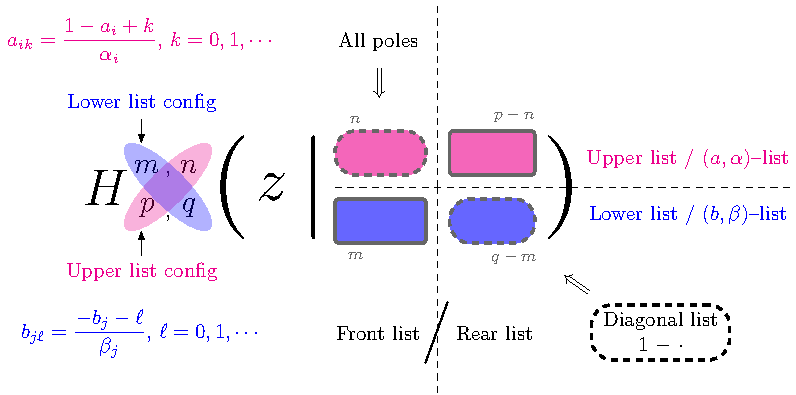
\includegraphics[width=1.0\textwidth]{./FoxH-Diagram.pdf}
  \caption{Diagram for the parameterization of the Fox $H$-function.}
  \label{F:Diagram}
\end{figure}
\bibliographystyle{alpha} \bibliography{refs.bib}
\end{document}

